\chapter{The Experimental Basis of Quantum Mechanics}
\label{ch:experiment}

Classical physics fails to explain blackbody radiation, the stability of atoms (Earnshaw's theorem forbids a stable static arrangement of charges), the optical spectra of atoms, and ferromagnetism. Quantum mechanics is hard because its effects are experimentally hard to access, it is computationally expensive (a system of $n$ two-state particles needs $2^n$ amplitudes), and it is hard to combine with gravity.

\begin{definition}[Planck's constant]
\[
    h = 6.626\times10^{-34}\ \text{J\,s},
    \qquad
    \hbar = \frac{h}{2\pi}.
\]
Its units, $[\text{J\,s}] = ML^2/T$, are those of energy$\times$time, momentum$\times$length, or angular momentum: $\hbar$ is an angular-momentum scale. Through it, a frequency ($1/\text{time}$) corresponds to an energy and a wavevector ($1/\text{length}$) to a momentum.
\end{definition}

\begin{fact}[Useful constants]
\[
    \alpha = \frac{e^2}{\hbar c}\approx\frac{1}{137},
    \qquad
    m_ec^2 = 0.511\ \text{MeV},
    \qquad
    \hbar c = 197.3\ \text{MeV\,fm},
    \qquad
    k_B = 1.38\times10^{-23}\ \text{J/K},
\]
with $e^2$ in Gaussian units ($e^2\to e^2/4\pi\varepsilon_0$ in SI).
\end{fact}

% ============================================================
\section{Blackbody Radiation and Heat Capacities}
% ============================================================

At thermal equilibrium, classical equipartition gives each quadratic degree of freedom an energy $k_BT/2$. In a cavity of length $L$, each standing EM mode $\lambda_n = 2L/n$, $\nu_n = cn/2L$, is such a degree of freedom, so the average energy is $\sum_{n\ge1}k_BT/2 = \infty$: the classical (Rayleigh--Jeans) spectrum grows without bound at high frequency, while the measured spectrum peaks and falls off.

\begin{fact}[Planck's resolution]
Light is made of quanta (photons) of energy $E_n = h\nu_n$. If $k_BT\gg E_n$ there are many photons in the mode and the classical answer holds. If $k_BT\ll E_n$, the mean number of photons is suppressed as $e^{-E_n/k_BT}$, so the energy
\[
    \langle E\rangle = \sum_{n\ge1}\sum_{k\ge0}E_nk\,\Pr[k\text{ photons at frequency }\nu_n] < \infty,
\]
in agreement with experiment.
\end{fact}

\begin{figure}[ht]
\centering
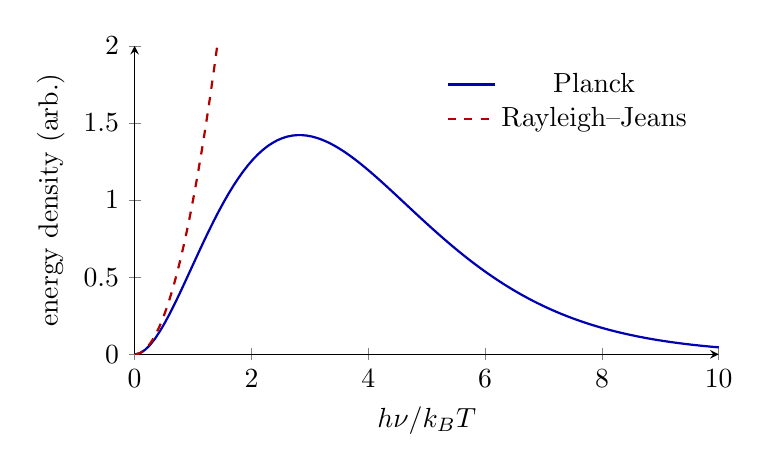
\begin{tikzpicture}
\begin{axis}[width=9cm,height=5.5cm,xlabel={$h\nu/k_BT$},ylabel={energy density (arb.)},xmin=0,xmax=10,ymin=0,ymax=2,axis lines=left,legend style={draw=none,at={(0.97,0.95)},anchor=north east},domain=0.01:10,samples=120]
\addplot[thick,blue!70!black]{x^3/(exp(x)-1)};
\addlegendentry{Planck}
\addplot[thick,dashed,red!70!black,domain=0.01:2.2]{x^2};
\addlegendentry{Rayleigh--Jeans}
\end{axis}
\end{tikzpicture}
\caption{Blackbody spectrum. The classical (Rayleigh--Jeans) result $\propto\nu^2$ agrees at low frequency but diverges; quantization suppresses modes with $h\nu\gg k_BT$.}
\end{figure}

The same idea explains the heat capacity of diatomic gases. Classically $C_V = k_B\cdot(\#\text{d.o.f.})/2$ per molecule: a monatomic gas has $C_V = \frac32Nk_B$, and a diatomic gas with 3 translational, 2 rotational and 2 vibrational (kinetic and potential) degrees of freedom should have $C_V = \frac72Nk_B$ at all temperatures. Measured, $C_V/Nk_B$ climbs in steps from $\frac32$ to $\frac52$ (around $10^2$\,K) to $\frac72$ (around $10^3$--$10^4$\,K): each degree of freedom has a characteristic energy it needs before it can be excited, and is frozen out below it.

\begin{formula}[Heisenberg uncertainty principle]
\[
    \Delta x\,\Delta p \ge \frac\hbar2 .
\]
\end{formula}

\begin{example}[Scale of quantum effects]
For a gas of rubidium atoms ($m = 87m_p$) in a 1\,cm box at room temperature, $\Delta p\approx\sqrt{mk_BT}\approx2.5\times10^{-23}$\,kg\,m/s, so $\Delta x\Delta p\approx4\times10^8\hbar$: thoroughly classical. Laser-cooled to $10^{-6}$\,K and trapped to $\Delta x\sim10^{-6}$\,m, $\Delta x\Delta p\sim2\hbar$, and quantum effects such as Bose--Einstein condensation appear.
\end{example}

% ============================================================
\section{Light as Particles}
% ============================================================

\subsection{The Mach--Zehnder Interferometer}

A classical EM wave $E_x = \mathrm{Re}\bigl[\alpha e^{i(\omega t-kz)}\bigr]$ with $\alpha = re^{i\phi}$ carries energy density $\propto|\alpha|^2$. Interference of two beams from the same source measures their relative phase. A beam splitter maps the amplitudes in its two input ports to its two output ports by a matrix,
\[
    \begin{pmatrix}\alpha'\\\beta'\end{pmatrix} = \begin{pmatrix}r&u\\t&v\end{pmatrix}\begin{pmatrix}\alpha\\\beta\end{pmatrix},
\]
and conservation of energy, $|\alpha'|^2+|\beta'|^2 = |\alpha|^2+|\beta|^2$, requires this matrix to be \emph{unitary}: $|r|^2+|t|^2 = 1$, $|u|^2+|v|^2 = 1$, and orthogonal columns, $ru^*+tv^* = 0$. A phase shifter acts as $\operatorname{diag}(1,e^{i\delta})$.

\begin{example}[Mach--Zehnder with single photons]
Use $\mathrm{BS1} = \frac{1}{\sqrt2}\begin{pmatrix}-1&1\\1&1\end{pmatrix}$ and $\mathrm{BS2} = \frac{1}{\sqrt2}\begin{pmatrix}1&1\\-1&1\end{pmatrix}$. Then
\[
    \mathrm{BS2}\cdot\mathrm{BS1} = \begin{pmatrix}0&1\\-1&0\end{pmatrix},
    \qquad
    \begin{pmatrix}1\\0\end{pmatrix}\mapsto\begin{pmatrix}0\\-1\end{pmatrix}:
\]
the photon always arrives at the bottom detector. For a single photon, the detector clicks with probability $|\text{amplitude}|^2$. The photon interferes destructively with itself: it cannot be only in the top or bottom arm, but has an amplitude in both. Blocking one arm destroys the interference, and each detector then clicks $1/4$ of the time (the block absorbs $1/2$).
\end{example}

\begin{example}[Elitzur--Vaidman bomb tester]
Put a bomb that explodes when hit by a photon in one arm. A dud bomb is transparent, so all photons reach $D_0$. A working bomb acts as a ``which-path'' measurement: it explodes with probability $1/2$, and otherwise the photon reaches $D_0$ or $D_1$ with probability $1/4$ each. A click at $D_1$ certifies a working bomb that did \emph{not} explode, which is impossible in any classical (``billiard ball'') model.
\end{example}

\subsection{The Photoelectric Effect}

Light of frequency $\nu$ on a metal ejects electrons. The stopping potential $V_0$ that halts the current measures the maximum kinetic energy, $K_{\max} = \frac12mv_{\max}^2 = eV_0$. The results contradict the wave picture:
\begin{enumerate}
    \item $K_{\max}$ is independent of intensity (over a $10^7$ range), though energy should grow with intensity.
    \item There is a cutoff frequency $\nu_0$, depending on the metal, below which no electrons are emitted at any intensity.
    \item There is no delay at very weak intensity, though classically the electron would need time to absorb enough energy.
\end{enumerate}

\begin{formula}[Einstein's photoelectric equation (1905)]
Light comes in quanta of energy $E = h\nu$, each photoelectron is ejected by one photon, and electrons are bound with minimum binding energy $W_0$ (the \emph{work function}). Then
\[
    K_{\max} = h\nu - W_0 = h(\nu-\nu_0),
    \qquad
    \nu_0 = W_0/h .
\]
\end{formula}
Increasing the intensity increases the rate of photons, and so the number of photoelectrons, but not $K_{\max}$; photons with $\nu<\nu_0$ cannot eject even the most weakly bound electrons. The slope of $K_{\max}(\nu)$ is the same $h$ found from thermal radiation.

\subsection{Compton Scattering}

Classically, light scatters off bound electrons at its own frequency (Rayleigh scattering, which makes the sky blue). Compton scattered monochromatic X-rays off graphite and measured the scattered wavelength by Bragg reflection ($n\lambda = 2d\sin\phi$). Besides the unshifted line (scattering from tightly bound electrons), a shifted line appears, increasingly shifted at larger angle. Treating the photon as a particle with $E = pc = h/\lambda$ scattering elastically off a free electron, conservation of energy and momentum give

\begin{formula}[Compton shift]
\[
    \Delta\lambda = \lambda_1 - \lambda_0 = \frac{h}{m_ec}(1-\cos\theta),
    \qquad
    \frac{h}{m_ec}\approx0.0243\ \text{\AA},
\]
largest, $2h/m_ec$, for backscattering ($\theta = \pi$).
\end{formula}

Quantum effects matter when $h\nu\gtrsim m_ec^2$ (Compton rather than Rayleigh scattering) and, for blackbody radiation, when $h\nu\gtrsim k_BT$.

\subsection{Bremsstrahlung}

Electrons accelerated through $V_0\sim5$--$50$\,kV and stopped in a target emit X-rays. Classically one expects a continuous spectrum spanning all wavelengths; instead there is a sharp short-wavelength cutoff. It is the photon carrying the electron's entire kinetic energy:
\[
    h\nu_{\max} = eV_0,
    \qquad
    \lambda_{\min} = \frac{hc}{eV_0}.
\]

\begin{formula}[Relativistic energy and momentum]
\[
    E = \gamma m_0c^2,
    \qquad
    \lvect{p} = \gamma m_0\lvect{v},
    \qquad
    E^2 = p^2c^2 + (m_0c^2)^2,
    \qquad
    \gamma = \frac{1}{\sqrt{1-v^2/c^2}},
\]
with rest energy $m_0c^2$, kinetic energy $K = (\gamma-1)m_0c^2\approx\frac12m_0v^2$, and $E = pc$ for a photon.
\end{formula}

% ============================================================
\section{Matter as Waves}
% ============================================================

Blackbody radiation, the photoelectric effect, bremsstrahlung and Compton scattering all show that light behaves as particles with $E = h\nu$ and $p = E/c = h/\lambda$. De Broglie proposed the converse.

\begin{formula}[de Broglie relation]
\[
    \lambda = \frac{h}{p}
\]
for all matter, not just photons.
\end{formula}

\begin{example}[de Broglie wavelengths]
A 10\,g stone moving at 10\,m/s has $\lambda\approx6.6\times10^{-24}$\,\AA. An electron with $K = 100$\,eV has $\lambda = h/\sqrt{2mK}\approx1.2$\,\AA, comparable to atomic sizes, so wave behaviour of matter is detectable at atomic scales.
\end{example}

\subsection{The Bohr Atom}

Rutherford's atom (size $\sim1$\,\AA, nucleus $\sim10^{-5}$\,\AA) has electrons orbiting a positive nucleus, but a classical accelerating charge radiates and spirals in. Bohr postulated:
\begin{enumerate}
    \item Bound electrons move in certain orbits, bound by the Coulomb potential.
    \item These discrete orbits are \emph{stationary states} in which the electron does not radiate.
    \item An electron moving between stationary states emits or absorbs a photon with $h\nu = E_i - E_f$.
    \item Orbital angular momentum is quantized, $L = n\hbar$.
\end{enumerate}
The last follows from de Broglie by fitting a whole number of wavelengths around the orbit: $2\pi r = n\lambda = nh/p$, so $L = rp = n\hbar$.

For a hydrogen-like atom (nuclear charge $Ze$, Gaussian units), $mv^2/r = Ze^2/r^2$ and $L = mvr = n\hbar$ give

\begin{formula}[Bohr atom]
\[
    r_n = \frac{n^2}{Z}\frac{\hbar^2}{me^2} = \frac{n^2}{Z}a_0,
    \qquad
    E_n = -\frac12\frac{Z^2e^4m}{n^2\hbar^2} = -\frac12mc^2\frac{(Z\alpha)^2}{n^2},
\]
with $a_0 = \hbar^2/me^2\approx0.53$\,\AA. For $Z = n = 1$, $E_1 = -13.6$\,eV, the ionization energy of hydrogen. Transitions give the Rydberg formula
\[
    \frac1\lambda = \frac{e^2}{2hca_0}\left(\frac{1}{n_f^2} - \frac{1}{n_i^2}\right),
\]
with the Lyman ($n_f = 1$), Balmer ($n_f = 2$) and Paschen ($n_f = 3$) series.
\end{formula}

\subsection{Wilson--Sommerfeld Quantization}

Planck quantized the energy of an oscillator and Bohr the angular momentum of an orbit: how do we know what to quantize? For a wave $e^{ikq}$ around a closed path, constructive interference requires the phase $\phi = \int k\,dq$ to advance by $2\pi n$. With $k = 2\pi/\lambda = 2\pi p/h$:

\begin{formula}[Wilson--Sommerfeld quantization rule (1916)]
\[
    \oint p\,dq = nh
\]
for any periodic system with coordinate $q$ and conjugate momentum $p$.
\end{formula}

\begin{example}[Harmonic oscillator]
For $E = p^2/2m + \frac12m\omega^2x^2$, the orbit in phase space is an ellipse with $p = m\omega\sqrt{x_{\max}^2-x^2}$, and
\[
    \oint p\,dx = 4m\omega\int_0^{x_{\max}}\sqrt{x_{\max}^2-x^2}\,dx = \pi m\omega x_{\max}^2 = \frac{2\pi E}{\omega} = nh,
\]
so $E_n = n\hbar\omega = nh\nu$: Planck's quantization.
\end{example}

\begin{example}[Bohr quantization in a quartic potential]
For circular orbits in $V = Ar^4$, the force balance $mr\omega^2 = 4Ar^3$ and $L = mr^2\omega = n\hbar$ give $r^6 = n^2\hbar^2/4Am$, and the energy $E = \frac12mr^2\omega^2 + Ar^4 = 3Ar^4$:
\[
    E_n = 3A\Bigl(\frac{n^2\hbar^2}{4Am}\Bigr)^{2/3}\propto n^{4/3}.
\]
\end{example}

% ============================================================
\section{The Double-Slit Experiment}
\label{sec:double-slit}
% ============================================================

Electrons from a source pass through slits $A$ and $B$, separated by $d$, and land on a screen a distance $L\gg d$ away. Let $P_A(y)$ be the distribution with only $A$ open, $P_B$ with only $B$, and $P_{AB}$ with both. Experimentally, $P_{AB}\neq P_A + P_B$; there are even points where $P_{AB} = 0$.

Describe the electron by a wavefunction with probability density $|\Psi|^2$. With both slits open, $\Psi_{AB} = \Psi_A + \Psi_B$, so
\[
    P_{AB} = |\Psi_A|^2 + |\Psi_B|^2 + 2\,\mathrm{Re}(\Psi_A^*\Psi_B),
\]
the last term being the interference. Taking $\Psi_{A,B} = Ce^{ikL_{A,B}}$ with path lengths $L_{A,B}\approx L + (y^2\mp yd)/2L$ for $d\ll y\ll L$,
\[
    |\Psi_{AB}|^2 = 4|C|^2\cos^2\Bigl(\frac{k\,yd}{2L}\Bigr),
\]
with peaks at $y_n = n\lambda L/d$. An extra relative phase $\phi_B-\phi_A$ shifts the pattern. Finite slit width supplies an envelope.

\begin{figure}[ht]
\centering
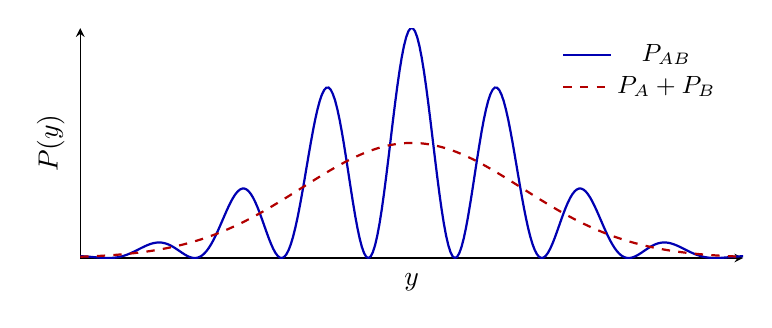
\begin{tikzpicture}
\begin{axis}[width=10cm,height=4.5cm,xlabel={$y$},ylabel={$P(y)$},axis lines=left,ytick=\empty,xtick=\empty,domain=-3:3,samples=300,ymin=0,legend style={draw=none,at={(0.98,0.98)},anchor=north east,font=\small}]
\addplot[thick,blue!70!black]{4*cos(deg(4*x))^2*exp(-x^2/2)};
\addlegendentry{$P_{AB}$}
\addplot[thick,dashed,red!70!black]{2*exp(-x^2/2)};
\addlegendentry{$P_A+P_B$}
\end{axis}
\end{tikzpicture}
\caption{Two-slit pattern. With both slits open the amplitudes add, giving fringes under the single-slit envelope; with which-path information the probabilities add and the fringes disappear.}
\end{figure}

\begin{fact}[Which-path information destroys interference]
If we determine which path the electron took, there is no interference and $P_{AB} = P_A + P_B$. To see the electron with light, the photon must resolve the slits, $\lambda_{\text{ph}}<d$, so it kicks the electron by $\Delta p_y\sim h/\lambda_{\text{ph}}$, which shifts its landing point by $\Delta y\sim\lambda_eL/\lambda_{\text{ph}}>\lambda_eL/d$: more than the fringe spacing, washing out the pattern. If the photon hits with probability $\pi$, the distribution is $\pi(P_A+P_B) + (1-\pi)P_{AB}$.
\end{fact}
